\documentclass[12pt,a4paper]{report}
\usepackage{amsmath}
\usepackage{amssymb}
\usepackage{hyperref}
\usepackage{graphicx}
\usepackage{geometry}
\usepackage[none]{hyphenat}
\usepackage{tikz}
\usepackage{float}
% Ensure valid float specifiers are used

\usetikzlibrary{external, shapes.geometric, arrows, arrows.meta, decorations.pathmorphing}
% \tikzexternalize % Enable TikZ externalization
\graphicspath{{images/}}

% Define python style for highlighting code
\usepackage{listings}
\definecolor{deepgray}{rgb}{0.4, 0.4, 0.4}
\usepackage{color}
\definecolor{deepblue}{rgb}{0,0,0.6}
\definecolor{deepred}{rgb}{0.6,0,0}
\definecolor{deepgreen}{rgb}{0,0.5,0}

% code RGB
\definecolor{codegreen}{rgb}{0,0.6,0}
\definecolor{codegray}{rgb}{0.5,0.5,0.5}
\definecolor{codepurple}{rgb}{0.58,0,0.82}
\definecolor{backcolour}{rgb}{0.95,0.95,0.92}

% Define python style for highlighting code
\lstdefinestyle{pythonstyle}{
    keywords={and, as, assert, break, class, continue, def, del, elif, else, except, False, finally, for, from, global, if, import, in, is, lambda, None, nonlocal, not, or, pass, raise, return, True, try, while, with, yield},
    keywordstyle=\color{deepblue}\bfseries,
    ndkeywords={self},
    ndkeywordstyle=\color{deepgray}\bfseries,
    identifierstyle=\color{black},
    sensitive=true,
    comment=[l]{\#},
    commentstyle=\color{deepgreen}\ttfamily,
    stringstyle=\color{deepred}\ttfamily,
    numberstyle=\tiny\color{gray},
    morestring=[b]',
    morestring=[b]``,
    basicstyle=\ttfamily,
    breakatwhitespace=false,
    breaklines=true,
    captionpos=b,
    keepspaces=true,
    numbers=left,
    numbersep=5pt,
    showspaces=false,
    showstringspaces=false,
    showtabs=false,
    tabsize=2
}

\lstdefinestyle{graystyle}{
    backgroundcolor=\color{backcolour},
    commentstyle=\color{codegreen},
    keywordstyle=\color{magenta},
    numberstyle=\tiny\color{codegray},
    stringstyle=\color{codepurple},
    basicstyle=\ttfamily,
    comment=[l]{\#},
    commentstyle=\color{deepgreen}\footnotesize\rmfamily,
    breakatwhitespace=false,
    breaklines=true,
    captionpos=b,
    keepspaces=true,
    numbers=left,
    numbersep=5pt,
    showspaces=false,
    showstringspaces=false,
    showtabs=false,
    tabsize=2,
    language=Python,
}

\lstset{style=graystyle}


\geometry{a4paper, margin=1in}

\title{Advantage of Quantum Computing in Breaking RSA Encryption}
\author{Srinivas Rao Tammireddy \\ Roll No: 217Y1A05C0 \\ Guide: Dr. S. Prathap Singh}
\date{\today}

\sloppy % Allow LaTeX to adjust spacing to avoid underfull hbox warnings
\hfuzz=99pt             % Increase tolerance for overfull hboxes
\hbadness=10000         % Suppress warnings for underfull hboxes


\begin{document}

\maketitle

\chapter*{Certificate}
This is to certify that the seminar report titled \textbf{Advantage of Quantum Computing in Breaking RSA Encryption} has been successfully completed by \textbf{Your Name}, Roll No: \textbf{Your Roll Number}, under the guidance of \textbf{Guide Name}. This report is submitted in partial fulfillment of the requirements for the seminar presentation.

\vspace{2cm}
\begin{flushright}
Signature of Guide \\
Signature of Student
\end{flushright}

\newpage

\tableofcontents
\listoffigures
\newpage

\chapter*{Abstract}
Quantum computing has emerged as a revolutionary paradigm in computation, offering significant advantages over classical computing for certain types of problems. One of the most notable implications of quantum computing is its potential to break widely used cryptographic systems, such as RSA encryption. This report explores the principles of RSA encryption, the capabilities of quantum computing, and how quantum algorithms, particularly Shor's algorithm, pose a threat to the security of RSA\@. The report also discusses the implications of this threat and the need for quantum-resistant cryptographic systems.
\chapter{Introduction to RSA Encryption and Quantum Computing}
\label{chap:introduction}
\sloppy
RSA encryption is a cornerstone of modern cryptography, widely used to secure digital communications. Its security is based on the computational difficulty of factoring large integers, a problem that classical computers find infeasible to solve within a reasonable timeframe. However, the advent of quantum computing introduces a paradigm shift in computational capabilities. Quantum computers, leveraging principles such as superposition and entanglement, can solve certain problems exponentially faster than classical computers. This chapter provides an overview of RSA encryption, its working principles, its critical role in ensuring secure communication, and the potential impact of quantum computing on its security.

\section{Overview of RSA Encryption}
RSA encryption, named after its inventors Rivest, Shamir, and Adleman, is a public-key cryptographic system that relies on two keys: a public key for encryption and a private key for decryption. The security of RSA is rooted in the mathematical challenge of factoring the product of two large prime numbers, which forms the basis of the private key.

\section{Working Principles of RSA}
The RSA algorithm involves three main steps:
\begin{enumerate}
    \item \textbf{Key Generation:} Two large prime numbers are chosen, and their product forms the modulus. The public and private keys are derived using modular arithmetic.
    \item \textbf{Encryption:} The sender uses the recipient's public key to encrypt the message, ensuring that only the recipient can decrypt it.
    \item \textbf{Decryption:} The recipient uses their private key to decrypt the message, recovering the original plaintext.
\end{enumerate}

\section{Role of RSA in Secure Communication}
RSA encryption is widely used in various applications, including:
\begin{itemize}
    \item Securing online transactions and communications.
    \item Authenticating digital signatures to verify the integrity of messages.
    \item Protecting sensitive data in email and file encryption.
\end{itemize}

\section{Introduction to Quantum Computing}
Quantum computing leverages the principles of quantum mechanics, such as superposition and entanglement, to perform computations. Unlike classical computers, which process information in binary bits, quantum computers use quantum bits (qubits) that can represent multiple states simultaneously.

\section{Impact of Quantum Computing on RSA}
The computational power of quantum computers poses a significant threat to RSA encryption. Quantum algorithms, such as Shor's algorithm, can factorize large integers exponentially faster than classical algorithms, rendering RSA insecure. This has profound implications for digital security and the need to develop quantum-resistant cryptographic systems.

This report will delve into the mathematical foundation of RSA encryption, the vulnerabilities of RSA to quantum attacks, and the implications of quantum computing on digital security. It will also explore the existing methods for breaking RSA encryption, the drawbacks of these methods, and the advantages of transitioning to quantum-resistant cryptographic systems. The report will conclude with a discussion on the future enhancements and applications of quantum-resistant cryptography.

\chapter{The Vulnerability of RSA Encryption to Quantum Computing: Literature Review}

\section{Introduction to RSA Vulnerability}
Rivest -- Shamir -- Adleman (RSA) encryption, a cornerstone of modern digital communication, provides security by transforming readable data into an unintelligible format that can only be reversed with a specific key~\cite{Okta}. This method relies on the computational difficulty of solving certain mathematical problems using classical computers~\cite{SecureW2}. However, as discussed in Chapter~\ref{chap:introduction}, the emergence of quantum computing presents a potential paradigm shift in computational power, threatening the security of widely used encryption algorithms like RSA~\cite{AuthoreaImplementation}. This chapter examines the fundamental principles of RSA encryption, the theoretical capability of quantum computers utilizing Shor's algorithm to compromise its security, the current state of quantum computing technology, the potential impact on cybersecurity, and the ongoing development of countermeasures in the form of post-quantum cryptography.

\section{RSA Encryption Fundamentals Review}
RSA is an asymmetric encryption algorithm that employs a pair of mathematically linked keys: a public key and a private key~\cite{SecureW2}. The public key is freely available and used for encrypting messages, while the private key is kept confidential by the owner and is necessary for decryption~\cite{SecureW2}. This system eliminates the need for prior key sharing, a significant advantage over traditional symmetric encryption methods~\cite{SplunkRSA}. 

The security of RSA hinges on the generation of these keys, which involves selecting two large prime numbers, denoted as \(p\) and \(q\)~\cite{SecureW2}. These primes are multiplied to produce a modulus \(n\), which forms part of both the public and private keys~\cite{SecureW2}. The public key consists of the pair \((n, e)\), where \(e\) is the encryption exponent. The private key includes \(n\) and a decryption exponent \(d\), which is the modular multiplicative inverse of \(e\) modulo \(\phi(n)\), where \(\phi(n)\) is Euler's totient function calculated as \((p - 1) \cdot (q - 1)\)~\cite{GeeksForGeeks}. 

Encryption involves raising the plaintext message \(m\) to the power of \(e\) and taking the modulus of \(n\) to obtain the ciphertext \(C\) (\(C = m^e \bmod n\))~\cite{GeeksForGeeks}. Decryption reverses this process by raising the ciphertext \(C\) to the power of \(d\) and taking the modulus of \(n\) to retrieve the original message \(m\) (\(m = C^d \bmod n\))~\cite{GeeksForGeeks}. This process is further illustrated in Chapter~\ref{sec:key_generation}.

\section{Mathematical Foundation of RSA Security Analysis}
The security of RSA encryption is fundamentally based on the computational difficulty of factoring large integers, specifically the modulus \(n\), back into its original prime factors \(p\) and \(q\)~\cite{SecureW2}. While multiplying two large prime numbers is a computationally straightforward task, reversing this process to find the prime factors of their product becomes exponentially harder as the size of the numbers increases~\cite{SecureW2}.

The RSA problem is defined as the task of recovering the original message given only the public key \((n, e)\) and the ciphertext~\cite{RSAWiki}. The most efficient known classical method to solve this problem involves factoring the modulus \(n\). The length of the RSA key, typically 1024 or 2048 bits, determines the size of the modulus \(n\). Larger key lengths result in significantly larger numbers, making factorization practically infeasible for classical computers within a reasonable timeframe~\cite{SecureW2}. For instance, factoring a 2048-bit number using classical methods would take an estimated 300 trillion years~\cite{ODUCommons}. This computational barrier is the cornerstone of RSA's security~\cite{SoftwareDominos}, as also discussed in Chapter~\ref{chap:existing_methods}.

\section{Shor's Algorithm: A Quantum Approach}
In 1994, Peter Shor developed a quantum algorithm that possesses the theoretical capability to factorize large integers exponentially faster than the best-known classical algorithms~\cite{SpinQShor}. Shor's algorithm leverages the principles of quantum mechanics, such as superposition and quantum parallelism, to perform computations in a fundamentally different way than classical computers~\cite{AuthoreaImplementation}. The principles of quantum mechanics underlying this algorithm are detailed in Chapter~\ref{chap:quantum_mechanics}.

The algorithm consists of two main stages: a classical reduction of the factorization problem to the problem of finding the period of a modular function, followed by the use of the Quantum Fourier Transform (QFT) on a quantum computer to efficiently determine this period~\cite{SpinQShor}. Once the period is found, the prime factors of the original number can be derived through classical post-processing using techniques like Euclid's algorithm to find the greatest common divisor~\cite{TechRxivImplementation}.

The ability of Shor's algorithm to solve the integer factorization problem in polynomial time poses a direct threat to the security of RSA encryption, as it could potentially allow an attacker with a sufficiently powerful quantum computer to efficiently derive the private key from the public key~\cite{SpinQShor}. This threat is further elaborated in Chapter~\ref{sec:key_generation}.

Quantum computers are not yet advanced enough to break RSA-2048 encryption due to limitations in stable qubits and error correction~\cite{SpinQShor, CatoNetworks}. Estimates suggest 4,000 to 20 million logical qubits are needed~\cite{BTQHowFar}. The largest number factored so far is 21~\cite{SpinQShor}, and hybrid approaches have only tackled very small keys~\cite{FreemindtronicRSA}. This aligns with the challenges in Chapter~\ref{sec:challenge_quantum_computing}.


\chapter{Background on RSA Encryption and Its Vulnerabilities}
The existing cryptographic systems, including RSA, rely on the computational difficulty of certain mathematical problems, such as integer factorization. Classical computers are unable to solve these problems efficiently, which forms the basis of RSA's security. This chapter discusses the existing system and its reliance on classical computational limitations.

\section{Mathematical Foundation of RSA}
The RSA cryptosystem, introduced by Rivest, Shamir, and Adleman in 1978~\cite{Rivest1978}, is based on the mathematical principles of number theory and modular arithmetic.

\section{Key Generation Process}
\label{sec:key_generation}
The RSA key generation process involves the following steps:
\begin{enumerate}
    \item Select two large prime numbers, \(p\) and \(q\) (typically 1024 bits or more).
    \item Compute their product, \(n = p \times q\), which serves as the modulus.
    \item Calculate the totient, \(\phi(n) = (p-1)(q-1)\).
    \item Choose a public exponent, \(e\), such that \(1 < e < \phi(n)\) and \(\gcd(e, \phi(n)) = 1\).
    \item Compute the private exponent, \(d\), as the modular multiplicative inverse of \(e\) modulo \(\phi(n)\), satisfying \(e \cdot d \equiv 1 \pmod{\phi(n)}\).
\end{enumerate}

As shown in Figure~\ref{fig:key_generation}, this process ensures the generation of secure keys for encryption and decryption.

\begin{figure}[ht!]
    \centering
    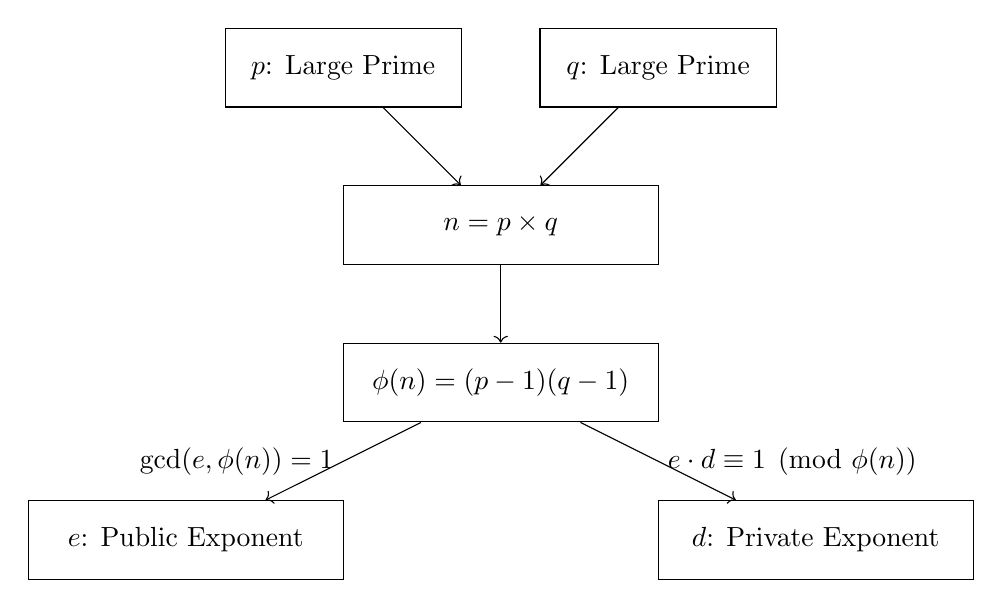
\begin{tikzpicture}
        % Draw the nodes
        \node[draw, rectangle, minimum width=3cm, minimum height=1cm] (p) at (0, 0) {\(p\): Large Prime};
        \node[draw, rectangle, minimum width=3cm, minimum height=1cm] (q) at (4, 0) {\(q\): Large Prime};
        \node[draw, rectangle, minimum width=4cm, minimum height=1cm] (n) at (2, -2) {\(n = p \times q\)};
        \node[draw, rectangle, minimum width=4cm, minimum height=1cm] (phi) at (2, -4) {\(\phi(n) = (p-1)(q-1)\)};
        \node[draw, rectangle, minimum width=4cm, minimum height=1cm] (e) at (-2, -6) {\(e\): Public Exponent};
        \node[draw, rectangle, minimum width=4cm, minimum height=1cm] (d) at (6, -6) {\(d\): Private Exponent};
        
        % Draw the arrows
        \draw[->] (p) -- (n);
        \draw[->] (q) -- (n);
        \draw[->] (n) -- (phi);
        \draw[->] (phi) -- (e) node[midway, left] {\(\gcd(e, \phi(n)) = 1\)};
        \draw[->] (phi) -- (d) node[midway, right] {\(e \cdot d \equiv 1 \pmod{\phi(n)}\)};
    \end{tikzpicture}
    \caption[Key Generation]{Diagram illustrating the RSA key generation process.}%
    \label{fig:key_generation}
\end{figure}

\section{Encryption and Decryption Methods}
To encrypt a message \( M \) using a public encryption key \((e, n)\), proceed as follows:
\begin{enumerate}
    \item Represent the message as an integer between \( 0 \) and \( n-1 \). For long messages, break them into blocks and represent each block as such an integer.
    \item Encrypt the message by raising it to the \( e \)-th power modulo \( n \):
    \[
    C \equiv M^e \pmod{n},
    \]
    where \( C \) is the ciphertext.
\end{enumerate}

To decrypt the ciphertext \( C \), use the private decryption key \((d, n)\) and compute:
\[
M \equiv C^d \pmod{n}.
\]

Figure~\ref{fig:encryption_decryption} illustrates the encryption and decryption process.

\begin{figure}[ht!]%
    \centering
    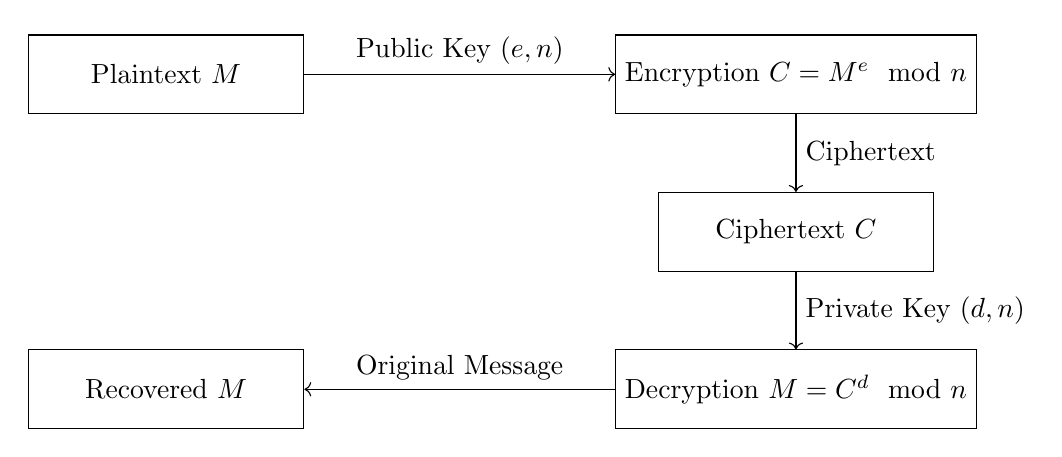
\begin{tikzpicture}
        % Nodes
        \node[draw, rectangle, minimum width=3.5cm, minimum height=1cm] (plaintext) at (0, 0) {Plaintext \(M\)};
        \node[draw, rectangle, minimum width=4.5cm, minimum height=1cm] (encryption) at (8, 0) {Encryption \(C = M^e \mod n\)};
        \node[draw, rectangle, minimum width=3.5cm, minimum height=1cm] (ciphertext) at (8, -2) {Ciphertext \(C\)};
        \node[draw, rectangle, minimum width=4.5cm, minimum height=1cm] (decryption) at (8, -4) {Decryption \(M = C^d \mod n\)};
        \node[draw, rectangle, minimum width=3.5cm, minimum height=1cm] (recovered) at (0, -4) {Recovered \(M\)};
        
        % Arrows
        \draw[->] (plaintext) -- (encryption) node[midway, above] {Public Key \((e, n)\)};
        \draw[->] (encryption) -- (ciphertext) node[midway, right] {Ciphertext};
        \draw[->] (ciphertext) -- (decryption) node[midway, right] {Private Key \((d, n)\)};
        \draw[->] (decryption) -- (recovered) node[midway, above] {Original Message};
        \end{tikzpicture}
    \caption[Encryption and Decryption]{Diagram illustrating the RSA encryption and decryption process.}%
    \label{fig:encryption_decryption}
\end{figure}

\section{Example: Encrypting a Message Using RSA}
To illustrate the RSA encryption process, consider the following example:

\subsection{Key Generation}
\begin{itemize}
    \item Choose two prime numbers: \( p = 17 \) and \( q = 19 \).
    \item Compute \( n = p \times q = 17 \times 19 = 323 \).
    \item Calculate the totient: \( \phi(n) = (p-1)(q-1) = 16 \times 18 = 288 \).
    \item Select a public exponent \( e = 5 \), such that \( 1 < e < \phi(n) \) and \( \gcd(e, \phi(n)) = 1 \).
    \item Compute the private exponent \( d \), satisfying \( e \cdot d \equiv 1 \pmod{\phi(n)} \). Using the extended Euclidean algorithm, \( d = 173 \).
\end{itemize}

The public key is \( (e, n) = (5, 323) \), and the private key is \( (d, n) = (173, 323) \).

\subsection{Encryption of the Message}
To encrypt the message \texttt{Hello}, convert each character to its ASCII equivalent:
\begin{itemize}
    \item \texttt{H} = 72, \texttt{e} = 101, \texttt{l} = 108, \texttt{o} = 111.
\end{itemize}

Message is represented as: \texttt{[72, 101, 108, 108, 111]}.

\subsection{Encryption of the Message}
To encrypt the message \texttt{Hello}, convert each character to its ASCII equivalent:
\begin{itemize}
    \item \texttt{H} = 72, \texttt{e} = 101, \texttt{l} = 108, \texttt{o} = 111.
\end{itemize}

Encrypt each character \( M \) using the formula:
\[
C \equiv M^e \pmod{n}.
\]

\begin{itemize}
    \item For \texttt{H}: \( C \equiv 72^5 \pmod{323} = 21 \).
    \item For \texttt{e}: \( C \equiv 101^5 \pmod{323} = 271 \).
    \item For \texttt{l}: \( C \equiv 108^5 \pmod{323} = 109 \).
    \item For \texttt{o}: \( C \equiv 111^5 \pmod{323} = 42 \).
\end{itemize}

The encrypted message is represented as:
\[
\text{Ciphertext: } \texttt{[21, 271, 109, 109, 42]}.
\]

The corresponding encrypted text is:
\[
\text{Encrypted Message: } \texttt{§ďmm*}.
\]

\subsection{Decryption of the Message}
To decrypt the ciphertext, use the private key \( (d, n) = (173, 323) \) and the formula:
\[
M \equiv C^d \pmod{n}.
\]

\begin{itemize}
    \item For \( C = 21 \): \( M \equiv 21^{173} \pmod{323} = 72 \) (\texttt{H}).
    \item For \( C = 271 \): \( M \equiv 271^{173} \pmod{323} = 101 \) (\texttt{e}).
    \item For \( C = 109 \): \( M \equiv 109^{173} \pmod{323} = 108 \) (\texttt{l}).
    \item For \( C = 42 \): \( M \equiv 42^{173} \pmod{323} = 111 \) (\texttt{o}).
\end{itemize}

The decrypted message is \texttt{Hello}, demonstrating the correctness of the RSA encryption and decryption process.

\section{Mathematical Proof of Correctness}
The correctness of the decryption process is guaranteed by Euler's theorem, which states:
\[
M^{\phi(n)} \equiv 1 \pmod{n},
\]
for any integer \( M \) coprime to \( n \). Here, \( \phi(n) \) is the Euler totient function, which gives the number of positive integers less than \( n \) that are relatively prime to \( n \). For prime numbers \( p \), we have:
\[
\phi(p) = p - 1.
\]

In the case of RSA, where \( n = p \cdot q \) (the product of two primes), the totient function is given by:
\[
\phi(n) = \phi(p) \cdot \phi(q) = (p - 1) \cdot (q - 1).
\]

Since \( d \) is chosen such that it is relatively prime to \( \phi(n) \), it has a multiplicative inverse \( e \) modulo \( \phi(n) \), satisfying:
\[
e \cdot d \equiv 1 \pmod{\phi(n)}.
\]

To prove the correctness of decryption, consider the encryption and decryption processes:
\[
D(E(M)) \equiv (E(M))^d \equiv (M^e)^d \pmod{n} = M^{e \cdot d} \pmod{n}.
\]

Using the property \( e \cdot d = k \cdot \phi(n) + 1 \) for some integer \( k \), we can rewrite:
\[
M^{e \cdot d} = M^{k \cdot \phi(n) + 1} \equiv M \pmod{n}.
\]

This follows from Euler's theorem, which ensures that \( M^{\phi(n)} \equiv 1 \pmod{n} \) for any \( M \) coprime to \( n \). Thus, the decryption process correctly recovers the original message \( M \).

Furthermore, for all \( M \), including cases where \( M \) is divisible by \( p \) or \( q \), the above equality holds due to the Chinese Remainder Theorem. Therefore, the encryption and decryption functions \( E \) and \( D \) are inverse permutations, ensuring the correctness of RSA~\cite{Rivest1978}.

\section{Very Large Primes in RSA}
The security of RSA encryption heavily relies on the use of very large prime numbers. These primes are chosen to ensure that the modulus \( n = p \times q \) is sufficiently large, making factorization computationally infeasible for classical computers.

\subsection{Properties of Large Primes}
Very large primes used in RSA have the following properties:
\begin{itemize}
    \item \textbf{Size:} Typically, primes are hundreds of digits long (e.g., 1024-bit, 2048-bit, or even larger primes in modern implementations). For example, a 200-digit \( n \) provides a strong margin of safety against classical attacks, while shorter lengths like 80 digits offer only moderate security.
    \item \textbf{Randomness:} Primes are generated randomly to avoid predictability, ensuring that attackers cannot guess or precompute potential primes.
    \item \textbf{Certainty:} Probabilistic primality tests, such as the Miller-Rabin test or the Baillie-PSW primality test, are used to ensure the numbers are prime with high confidence. Deterministic tests like the AKS primality test may also be used for absolute certainty, though they are computationally more expensive.
\end{itemize}

\subsection{Generation of Large Primes}
The process of generating large primes involves the following steps:
\begin{enumerate}
    \item \textbf{Random Selection:} Randomly select a large odd number within the desired range (e.g., 1024-bit or 2048-bit range).
    \item \textbf{Primality Testing:} Test the number for primality using efficient algorithms:
    \begin{itemize}
        \item \textbf{Miller-Rabin Test:} A probabilistic test that can quickly identify composite numbers. Multiple iterations increase the confidence level.
        \item \textbf{Lucas-Lehmer Test:} Often used for specific types of primes, such as Mersenne primes.
        \item \textbf{AKS Primality Test:} A deterministic test that guarantees correctness but is slower than probabilistic methods.
    \end{itemize}
    \item \textbf{Iteration:} If the number fails the primality test, repeat the process with a new candidate until a prime is found.
\end{enumerate}

\subsection{Challenges with Large Primes}
While the use of very large primes is essential for RSA security, it introduces several challenges:
\begin{itemize}
    \item \textbf{Computational Cost:} Generating and verifying large primes is computationally expensive, especially for key sizes of 4096 bits or more.
    \item \textbf{Storage and Transmission:} Large primes require more storage space and bandwidth for secure transmission, increasing the overhead in cryptographic systems.
    \item \textbf{Quantum Threats:} Despite the use of very large primes, RSA remains vulnerable to quantum algorithms like Shor's algorithm, which can efficiently factorize the modulus \( n \) and compromise the encryption.
\end{itemize}

\subsection{Importance of Large Primes in RSA}
Large primes are crucial for RSA's security, as factoring their product is computationally hard for classical methods. However, quantum computing's rise demands quantum-resistant cryptography to counter vulnerabilities from quantum algorithms.

\section{Python Implementation of RSA Encryption and Decryption}
The following Python code demonstrates the RSA encryption and decryption process using two different approaches:

\subsection{Generic RSA Implementation}
Listing~\ref{lst:rsa_example_generic} provides a generic implementation of RSA encryption and decryption in Python. It includes functions for key generation, encryption, and decryption, showcasing the mathematical principles of RSA.

\begin{itemize}
    \item The \texttt{generate\_keys} function generates public and private keys using two prime numbers.
    \item The \texttt{encrypt} function encrypts a plaintext message using the public key.
    \item The \texttt{decrypt} function decrypts the ciphertext using the private key.
\end{itemize}
\sloppy
This implementation demonstrates the core concepts of RSA and is suitable for educational purposes.

\hyphenpenalty=50
\exhyphenpenalty=50
\begin{lstlisting}[language=Python, caption=RSA Encryption and Decryption Example (Python 3.8+), label={lst:rsa_example_generic}]
import random  # Random module for key generation
from math import gcd  # GCD function for coprime check
from sympy import mod_inverse  # Modular inverse calculation
# Function to compute modular exponentiation
def mod_exp(base, exp, mod):
    result = 1
    while exp > 0:
        if exp % 2 == 1:  # If exponent is odd
            result = (result * base) % mod
        base = (base * base) % mod
        exp //= 2
    return result

# Function to generate RSA keys
def generate_keys(p, q):
    n, phi = p * q, (p - 1) * (q - 1)
    e = random.randrange(2, phi)
    while gcd(e, phi) != 1:
        e = random.randrange(2, phi)
    d = mod_inverse(e, phi)
    return (e, n), (d, n)  # Public key, Private key

# RSA Encryption
def encrypt(message, public_key):
    e, n = public_key
    return [mod_exp(ord(char), e, n) for char in message]

# RSA Decryption
def decrypt(ciphertext, private_key):
    d, n = private_key
    return ''.join([chr(mod_exp(char, d, n)) for char in ciphertext])

# Example Usage
p = int(input("Enter a prime number p: "))
q = int(input("Enter a prime number q: "))
public_key, private_key = generate_keys(p, q)

message = "HELLO"
print("Original Message:", message)
print("Encrypted Message:", encrypt(message, public_key))
print("Decrypted Message:", decrypt(ciphertext, private_key))
\end{lstlisting}

\hyphenpenalty=10000
\exhyphenpenalty=10000

\subsection{Cryptography Library-Based Implementation}
Listing~\ref{lst:rsa_example} demonstrates an RSA implementation using the \texttt{cryptography} library in Python. This approach leverages built-in functions for key generation, encryption, and decryption, providing a more secure and efficient solution. For more details, refer to the official documentation at \href{https://cryptography.io/en/latest/hazmat/primitives/asymmetric/rsa/#}{cryptography}.

\begin{itemize}
    \item The {\texttt{generate\_rsa\_keys}} function generates RSA key pairs and serializes them in PEM format.
    \item The \texttt{encrypt\_message} function encrypts a message using the public key and OAEP padding.
    \item The \texttt{decrypt\_message} function decrypts the ciphertext using the private key and OAEP padding.
\end{itemize}

This implementation is suitable for real-world applications, as it adheres to modern cryptographic standards.

\subsubsection{Library Installation}
To use the \texttt{cryptography} library, install it using the following command:
\begin{lstlisting}[language=bash]
pip install cryptography
\end{lstlisting}

\subsubsection{Advantages of Using the \texttt{cryptography} Library}
\begin{itemize}
    \item \textbf{Security:} The library adheres to modern cryptographic standards, ensuring robust security for encryption and decryption.
    \item \textbf{Ease of Use:} Provides high-level APIs for common cryptographic operations, reducing the complexity of implementation.
    \item \textbf{Performance:} Optimized for performance, making it suitable for real-world applications.
    \item \textbf{Community Support:} Actively maintained and widely used, ensuring reliability and access to community resources.
\end{itemize}

\hyphenpenalty=50
\exhyphenpenalty=50
\begin{lstlisting}[language=Python, caption=Python code for RSA encryption and decryption, label={lst:rsa_example}]
from cryptography.hazmat.primitives.asymmetric import rsa, padding
from cryptography.hazmat.primitives import serialization, hashes

def generate_rsa_keys() -> tuple[bytes, bytes]:
    '''
    Generate RSA public and private keys.

    Returns:
        tuple[bytes, bytes]: A tuple containing the private key and public key in PEM format.
    '''
    private_key = rsa.generate_private_key(
        public_exponent=65537,
        key_size=2048
    )
    public_key = private_key.public_key()
    return (
        private_key.private_bytes(
            encoding=serialization.Encoding.PEM,
            format=serialization.PrivateFormat.PKCS8,
            encryption_algorithm=serialization.NoEncryption()
        ),
        public_key.public_bytes(
            encoding=serialization.Encoding.PEM,
            format=serialization.PublicFormat.SubjectPublicKeyInfo
        )
    )
def encrypt_message(public_key_pem: bytes, message: bytes) -> bytes:
    '''
    Encrypt a message using an RSA public key.

    Args:
        public_key_pem (bytes): The public key in PEM format.
        message (bytes): The plaintext message to encrypt.

    Returns:
        bytes: The encrypted ciphertext.
    '''
    public_key = serialization.load_pem_public_key(public_key_pem)
    return public_key.encrypt(
        message,
        padding.OAEP(
            mgf=padding.MGF1(algorithm=hashes.SHA256()),
            algorithm=hashes.SHA256(),
            label=None
        )
    )

def decrypt_message(private_key_pem: bytes, ciphertext: bytes) -> bytes:
    '''
    Decrypt a ciphertext using an RSA private key.

    Args:
        private_key_pem (bytes): The private key in PEM format.
        ciphertext (bytes): The encrypted ciphertext to decrypt.

    Returns:
        bytes: The decrypted plaintext message.
    '''
    private_key = serialization.load_pem_private_key(private_key_pem, password=None)
    return private_key.decrypt(
        ciphertext,
        padding.OAEP(
            mgf=padding.MGF1(algorithm=hashes.SHA256()),
            algorithm=hashes.SHA256(),
            label=None
        )
    )

# Example usage
private_key_pem, public_key_pem = generate_rsa_keys()
message = b"Hello, Quantum World!"
ciphertext = encrypt_message(public_key_pem, message)
decrypted_message = decrypt_message(private_key_pem, ciphertext)

# Print results
print("Original Message:", message)
print("Encrypted Message:", ciphertext)
print("Decrypted Message:", decrypted_message)
\end{lstlisting}
\hyphenpenalty=10000
\exhyphenpenalty=10000

\section{Vulnerabilities of RSA}
While RSA is secure against classical attacks with sufficiently large key sizes, it has inherent vulnerabilities:
\begin{itemize}
    \item \textbf{Small Key Sizes:} RSA keys smaller than 2048 bits are susceptible to factorization using advanced classical algorithms.
    \item \textbf{Implementation Flaws:} Poor implementation practices, such as weak random number generation, can compromise RSA security.
    \item \textbf{Side-Channel Attacks:} Physical attacks exploiting timing, power, or electromagnetic emissions can reveal private keys.
    \item \textbf{Quantum Threats:} The advent of quantum computing introduces algorithms, such as Shor's algorithm, that can efficiently factorize large integers, rendering RSA insecure.
\end{itemize}

\section{Mitigation Strategies}
To address these vulnerabilities, several strategies have been proposed:
\begin{itemize}
    \item \textbf{Increasing Key Sizes:} Using larger key sizes (e.g., 4096 bits) to enhance resistance against classical attacks.
    \item \textbf{Implementing Countermeasures:} Employing constant-time algorithms and secure random number generators to prevent side-channel attacks.
    \item \textbf{Transitioning to Quantum-Resistant Cryptography:} Developing and adopting cryptographic systems that are secure against quantum attacks.
\end{itemize}

\chapter{Quantum Mechanics and Its Role in Quantum Computing}
\label{chap:quantum_mechanics}
Quantum mechanics is the branch of physics that describes the behavior of matter and energy at the smallest scales, such as atoms and subatomic particles. It forms the theoretical foundation of quantum computing, enabling the development of algorithms that outperform classical counterparts for specific problems.

\section{Principles of Quantum Mechanics}
Quantum mechanics is governed by several key principles that distinguish it from classical physics:

\subsection{Quantization of Physical Properties}
Quantization is a fundamental concept in quantum mechanics, where certain physical properties, such as energy, angular momentum, and charge, can only take on discrete values. This is in contrast to classical mechanics, where these properties are continuous.

\subsubsection{Energy Quantization}
In quantum systems, energy levels are quantized, meaning that a particle can only occupy specific energy states. For example, the energy levels of an electron in a hydrogen atom are given by:
\[
E_n = -\frac{13.6 \, \text{eV}}{n^2},
\]
where \( n \) is a positive integer representing the principal quantum number. Here, \( 13.6 \, \text{eV} \) is the ionization energy of the hydrogen atom, which corresponds to the energy required to remove an electron from the ground state (\( n = 1 \)) to infinity (\( n \to \infty \)).

\begin{figure}[H]
    \centering
    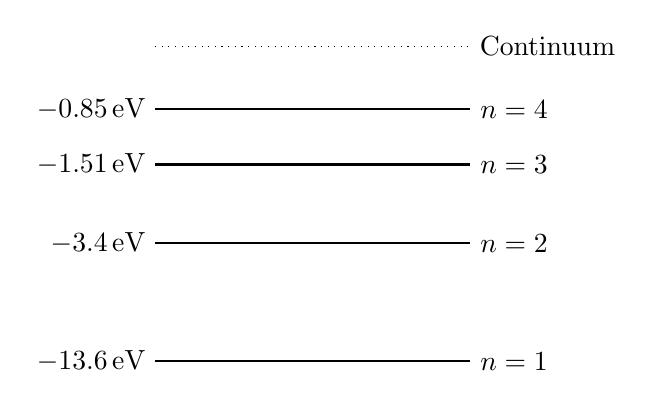
\begin{tikzpicture}
        % Energy levels
        \draw[thick] (0,0) -- (4,0) node[right] {\( n = 1 \)};
        \draw[thick] (0,1.5) -- (4,1.5) node[right] {\( n = 2 \)};
        \draw[thick] (0,2.5) -- (4,2.5) node[right] {\( n = 3 \)};
        \draw[thick] (0,3.2) -- (4,3.2) node[right] {\( n = 4 \)};
        \draw[dotted] (0,4) -- (4,4) node[right] {Continuum};
        % Labels
        \node[left] at (0,0) {\(-13.6 \, \text{eV}\)};
        \node[left] at (0,1.5) {\(-3.4 \, \text{eV}\)};
        \node[left] at (0,2.5) {\(-1.51 \, \text{eV}\)};
        \node[left] at (0,3.2) {\(-0.85 \, \text{eV}\)};
    \end{tikzpicture}
    \caption{Discrete energy levels of an electron in a hydrogen atom.}
\end{figure}

\subsubsection{Angular Momentum Quantization}
The angular momentum of a particle is also quantized. For example, the magnitude of the angular momentum of an electron in an atom is given by:
\[
L = \sqrt{\ell(\ell + 1)} \hbar,
\]
where \( \ell \) is the orbital quantum number, and \( \hbar \) is the reduced Planck's constant.

\subsubsection{Charge Quantization}
Electric charge is quantized in units of the elementary charge \( e \). For example, the charge of an electron is \( -e \), and the charge of a proton is \( +e \).

Quantization is a cornerstone of quantum mechanics, providing the framework for understanding the discrete nature of physical phenomena at microscopic scales.

\subsection{Wave-Particle Duality}
Wave-particle duality is a fundamental concept in quantum mechanics, stating that quantum entities, such as electrons and photons, exhibit both wave-like and particle-like behavior depending on the experimental setup. For example, in the double-slit experiment, particles like electrons create an interference pattern when not observed, demonstrating wave-like behavior. However, when observed, they behave like particles, striking specific locations on a detector.

\begin{figure}[H]
    \centering
    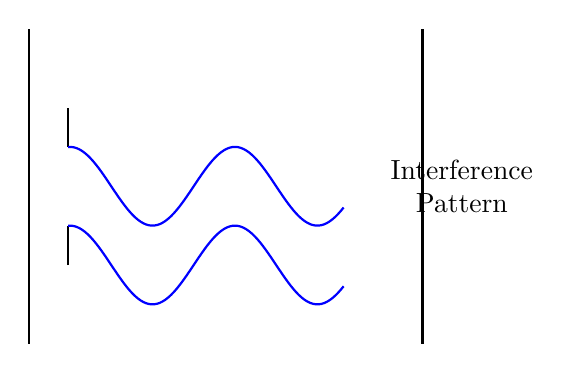
\begin{tikzpicture}
        % Slits
        \draw[thick] (0,0) -- (0,4);
        \draw[thick] (0.5,1) -- (0.5,1.5);
        \draw[thick] (0.5,2.5) -- (0.5,3);
        % Waves
        \draw[thick, blue, domain=0.5:4, samples=100] plot (\x, {2 + 0.5*sin(3*\x r)});
        \draw[thick, blue, domain=0.5:4, samples=100] plot (\x, {1 + 0.5*sin(3*\x r)});
        % Detector
        \draw[thick] (5,0) -- (5,4);
        \node[align=center] at (5.5,2) {Interference \\ Pattern};
    \end{tikzpicture}
    \caption{Wave-particle duality demonstrated in the double-slit experiment.}
\end{figure}

\subsection{Uncertainty Principle (Heisenberg's Principle)}
The uncertainty principle, formulated by Werner Heisenberg, is a fundamental concept in quantum mechanics. It states that certain pairs of physical properties, such as position (\(x\)) and momentum (\(p\)), cannot be simultaneously measured with arbitrary precision. Mathematically, the principle is expressed as:
\[
\Delta x \cdot \Delta p \geq \frac{\hbar}{2},
\]
\begin{figure}[H]
     \centering
        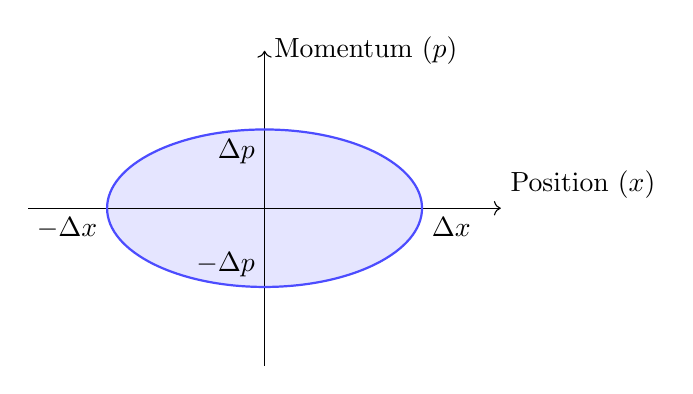
\begin{tikzpicture}
            % Uncertainty ellipse
            \fill[blue!10] (0,0) ellipse (2 and 1);
            
            % Axes
            \draw[->] (-3,0) -- (3,0) node[anchor=south west] {Position (\(x\))};
            \draw[->] (0,-2) -- (0,2) node[anchor=west] {Momentum (\(p\))};
            
            % Uncertainty ellipse with soft shading
            \draw[thick, blue!70] (0,0) ellipse (2 and 1);
            
            % Labels for axes
            \node[anchor=north east] at (-2,0) {\(-\Delta x\)};
            \node[anchor=north west] at (2,0) {\(\Delta x\)};
            \node[anchor=south east] at (0,-1) {\(-\Delta p\)};
            \node[anchor=north east] at (0,1) {\(\Delta p\)};
        \end{tikzpicture}
        \caption[Uncertainty Principle]{Graphical representation of the uncertainty principle. The softly shaded ellipse illustrates the trade-off between uncertainties in position (\(x\)) and momentum (\(p\)).}
\end{figure}

\subsubsection{Implications of the Uncertainty Principle}
The uncertainty principle has profound implications for quantum mechanics:
\begin{itemize}
    \item \textbf{Wave-Particle Duality:} It highlights the wave-like nature of particles, as the position and momentum cannot be precisely defined simultaneously.
    \item \textbf{Quantum Systems:} It imposes fundamental limits on the precision of measurements in quantum systems, influencing the design of experiments and technologies like quantum computing.
    \item \textbf{Non-Deterministic Nature:} It underscores the probabilistic nature of quantum mechanics, where outcomes are described by probabilities rather than certainties.
\end{itemize}

\subsection{Wavefunction and Schrödinger's Equation}
The wavefunction \( |\psi\rangle \) describes the quantum state of a system and contains all the information about the system. The time evolution of the wavefunction is governed by the Schrödinger equation:
\[
i\hbar \frac{\partial}{\partial t} |\psi(t)\rangle = \hat{H} |\psi(t)\rangle,
\]
\begin{figure}[H]
    \centering    
    \resizebox{\linewidth}{!}{%
    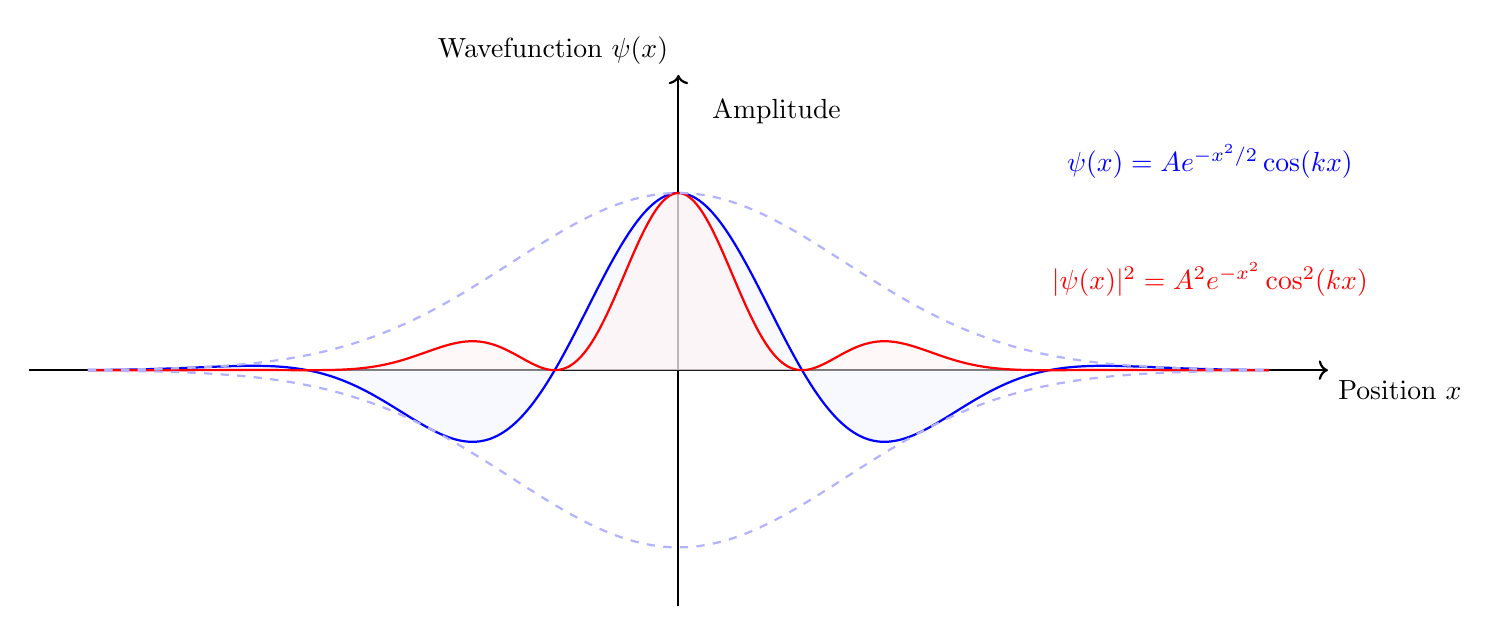
\begin{tikzpicture}[scale=1.5, line width=0.8pt]
        % Axes
        \draw[->] (-5.5, 0) -- (5.5, 0) node[anchor=north west] {Position \(x\)};
        \draw[->] (0, -2) -- (0, 2.5) node[anchor=south east] {Wavefunction \(\psi(x)\)};

        % Wavefunction
        \fill[blue!5, opacity=0.5] 
            (-5, 0) -- plot[domain=-5:5, samples=200] (\x, {1.5 * exp(-0.25 * \x * \x) * cos(1.5 * \x r)}) -- (5, 0) -- cycle;
        \draw[thick, blue, smooth, domain=-5:5, samples=200] 
            plot (\x, {1.5 * exp(-0.25 * \x * \x) * cos(1.5 * \x r)});

        % Dashed lines for probability density (\(\psi(x)^2\))
        \fill[red!5, opacity=0.5] 
            (-5, 0) -- plot[domain=-5:5, samples=200] (\x, {1.5 * exp(-0.5 * \x * \x) * cos(1.5 * \x r) * cos(1.5 * \x r)}) -- (5, 0) -- cycle;
        \draw[thick, red, smooth, domain=-5:5, samples=200] 
            plot (\x, {1.5 * exp(-0.5 * \x * \x) * cos(1.5 * \x r) * cos(1.5 * \x r)});

        % Dashed Gaussian envelope
        \draw[dashed, blue!30, domain=-5:5, samples=200] plot (\x, {1.5 * exp(-0.25 * \x * \x)});
        \draw[dashed, blue!30, domain=-5:5, samples=200] plot (\x, {-1.5 * exp(-0.25 * \x * \x)});

        % Labels
        \node[anchor=north, blue] at (4.5, 2) {\(\psi(x) = A e^{-x^2/2} \cos(kx)\)};
        \node[anchor=north, red] at (4.5, 1) {\(|\psi(x)|^2 = A^2 e^{-x^2} \cos^2(kx)\)};
        \node[anchor=south west] at (0.2, 2) {Amplitude};
    \end{tikzpicture}
    }
    \caption[schrodinger Wavefunction]{High-resolution wavefunction \(\psi(x)\) with a Gaussian envelope modulated by a cosine wave, and its probability density \(|\psi(x)|^2\) filled.}
    \label{fig:wavefunction_highend}
\end{figure}

\begin{figure}[H]
    \centering
    \resizebox{\linewidth}{!}{%
        \begin{tikzpicture}[scale=1.5, line width=0.8pt]
            % Axes
            \draw[->] (-4.5, 0) -- (4.5, 0) node[anchor=north west] {Position \(x\)};
            \draw[->] (0, -2) -- (0, 2.5) node[anchor=south east] {Potential \(V(x)\)};
            
            % Potential well
            \draw[thick, red, smooth] (-4, 2) -- (-1, 2) -- (-1, 0) -- (1, 0) -- (1, 2) -- (4, 2);
            \node[anchor=north] at (4.5, 2.2) {Potential \(V(x)\)};
            
            % Wavefunction inside well
            \draw[thick, blue, smooth, domain=-1:1, samples=200] 
                plot (\x, {1.8 * cos(3.14 * \x r)});
            
            % Dashed lines for boundaries
            \draw[dashed, gray] (-1, -2) -- (-1, 2);
            \draw[dashed, gray] (1, -2) -- (1, 2);
            
            % Labels for boundaries
            \node[anchor=north] at (-1, -2.2) {\(-a\)};
            \node[anchor=north] at (1, -2.2) {\(a\)};
            
            % Additional labels
            \node[anchor=north west] at (0.2, 2.5) {Wavefunction \(\psi(x)\)};
            \node[anchor=north east] at (-4, -1.8) {Potential Well};
            
            % Energy level
            \draw[dotted, thick, green!70!black] (-1, 1) -- (1, 1);
            \node[anchor=west, green!70!black] at (1.2, 1) {Energy Level \(E_1\)};
        \end{tikzpicture}
    }
    \caption{High-resolution wavefunction \(\psi(x)\) in a potential well \(V(x)\).}
    \label{fig:schrodinger_highend}
\end{figure}

Solving the Schrödinger equation provides the wavefunction \( |\psi(t)\rangle \) at any given time, enabling the prediction of quantum behavior.

\subsection{Superposition Principle}
Superposition is a fundamental principle of quantum mechanics that allows quantum systems to exist in multiple states simultaneously. In the context of quantum computing, a quantum bit (qubit) can represent both \( |0\rangle \) and \( |1\rangle \) at the same time, unlike classical bits that can only represent one state at a time. Mathematically, a qubit in superposition is represented as:
\[
|\psi\rangle = \alpha |0\rangle + \beta |1\rangle,
\]
where \( \alpha \) and \( \beta \) are complex numbers satisfying \( |\alpha|^2 + |\beta|^2 = 1 \). This property enables quantum computers to process a vast number of possibilities simultaneously, leading to exponential speedups for certain types of problems.
\begin{figure}[H]
    \centering
        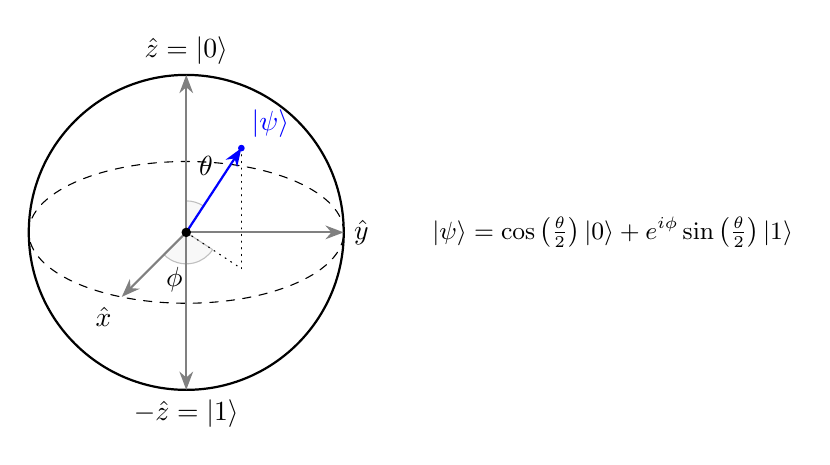
\begin{tikzpicture}[line cap=round, line join=round, >=Stealth]
        
        % Draw the outer sphere
        \draw[thick] (0,0) circle (2cm);
        
        % Draw the equatorial plane (dashed ellipse)
        \draw[dash pattern=on 3pt off 3pt] (0,0) ellipse (2cm and 0.9cm);
        
        % Highlight angles
        \draw[shift={(0,0)}, lightgray, fill, fill opacity=0.1] (0,0) -- (56.7:0.4) arc (56.7:90:0.4) -- cycle;
        \draw[shift={(0,0)}, lightgray, fill, fill opacity=0.1] (0,0) -- (-135.7:0.4) arc (-135.7:-33.2:0.4) -- cycle;
        
        % Axes
        \draw[->, thick, gray] (0,0) -- (0,2) node[anchor=south, black] {$\hat{z}=|0\rangle$};
        \draw[->, thick, gray] (0,0) -- (2,0) node[anchor=west, black] {$\hat{y}$};
        \draw[->, thick, gray] (0,0) -- ({-1.158*sin(45)},{-1.158*sin(45)}) node[anchor=north east, black] {$\hat{x}$};
        \draw[->, thick, gray] (0,0) -- (0,-2) node[anchor=north, black] {$-\hat{z}=|1\rangle$};
        
        % Qubit state vector
        \draw[thick, ->, blue] (0,0) -- (0.7,1.07) node[anchor=south west] {$|\psi\rangle$};
        
        % Projection lines
        \draw[dotted] (0.7,1.07) -- (0.7,-0.46);
        \draw[dotted] (0,0) -- (0.7,-0.46);
        
        % Angle labels
        \node at (-0.15,-0.6) {$\phi$};
        \node at (0.25,0.85) {$\theta$}; % Adjusted theta position slightly to the right
        
        % State label moved to the side
        \node[align=left, font=\small, anchor=west] at (3,0) {$|\psi\rangle = \cos\left(\frac{\theta}{2}\right)|0\rangle + e^{i\phi}\sin\left(\frac{\theta}{2}\right)|1\rangle$};
        
        % Markers
        \draw[fill] (0,0) circle (1.5pt); % Origin
        \draw[fill, blue] (0.7,1.07) circle (1pt); % Qubit state
    \end{tikzpicture}
    \caption{Representation of a qubit on the Bloch sphere, showing the state \( |\psi\rangle = \cos\left(\frac{\theta}{2}\right)|0\rangle + e^{i\phi}\sin\left(\frac{\theta}{2}\right)|1\rangle \) with angles \( \theta \) and \( \phi \). The vector \( |\psi\rangle \) is shown in blue, illustrating that the atom is in a superposition of states \( |0\rangle \) and \( |1\rangle \) simultaneously.}
    \end{figure}

\begin{figure}[H]
    \centering
    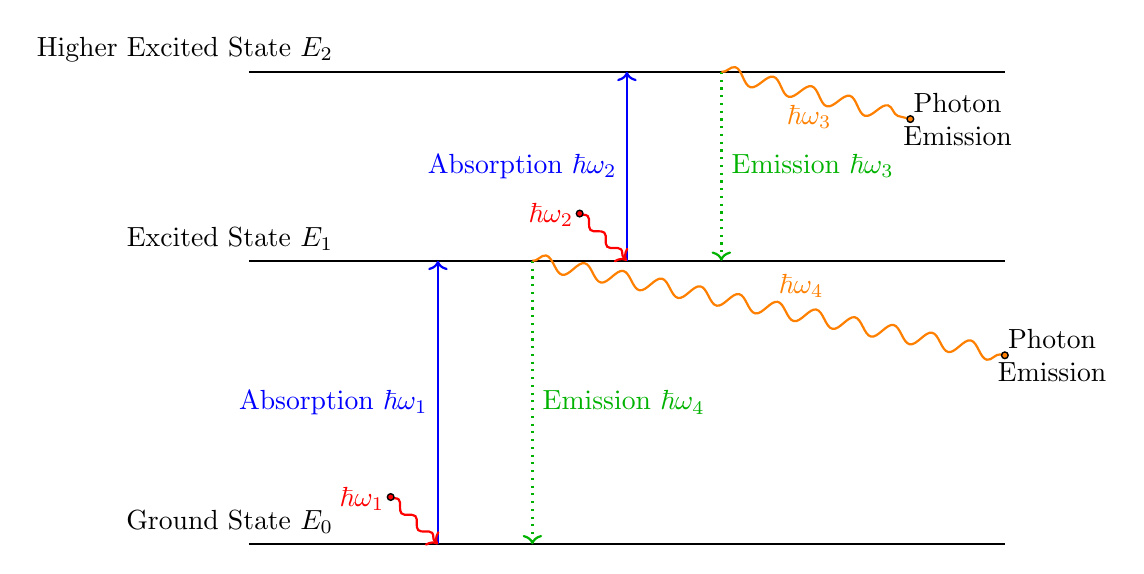
\begin{tikzpicture}[line width=0.8pt, scale=1.2]
        % Energy levels
        \draw[thick] (0,0) -- (8,0) node[above, near start, anchor=south east, xshift=-1.2cm] {Ground State \(E_0\)};
        \draw[thick] (0,3) -- (8,3) node[above, near start, anchor=south east, xshift=-1.2cm] {Excited State \(E_1\)};
        \draw[thick] (0,5) -- (8,5) node[above, near start, anchor=south east, xshift=-1.2cm] {Higher Excited State \(E_2\)};
        
        % Electron transitions (absorption)
        \draw[->, thick, blue] (2,0) -- (2,3) node[midway, left] {Absorption \(\hbar\omega_1\)};
        \draw[->, thick, blue] (4,3) -- (4,5) node[midway, left] {Absorption \(\hbar\omega_2\)};
        
        % Enhanced photon representations (incident photons with wave patterns)
        \draw[->, thick, red, decorate, decoration={snake, amplitude=0.5mm, segment length=3mm}] (1.5,0.5) -- (2,0) node[midway, above left, xshift=-2.5mm] {\(\hbar\omega_1\)};
        \draw[line width=0.5pt, fill=red] (1.5,0.5) circle (1pt);
        \draw[->, thick, red, decorate, decoration={snake, amplitude=0.5mm, segment length=3mm}] (3.5,3.5) -- (4,3) node[midway, above left, xshift=-2.5mm] {\(\hbar\omega_2\)};           
        \draw[line width=0.5pt, fill=red] (3.5,3.5) circle (1pt);
        
        % Relaxation paths (emission)
        \draw[->, thick, green!70!black, dotted] (5,5) -- (5,3) node[midway, right] {Emission \(\hbar\omega_3\)};
        \draw[->, thick, green!70!black, dotted] (3,3) -- (3,0) node[midway, right] {Emission \(\hbar\omega_4\)};
        
        % Wavy photon emission lines
        \draw[decorate, decoration={snake, amplitude=1mm, segment length=5mm}, thick, orange] (5,5) -- (7,4.5) node[midway, below right, xshift=-5mm] {\(\hbar\omega_3\)};
        \draw[line width=0.5pt, fill=orange] (7,4.5) circle (1pt);
        \draw[decorate, decoration={snake, amplitude=1mm, segment length=5mm}, thick, orange] (3,3) -- (8,2) node[midway, above right] {\(\hbar\omega_4\)};
        \draw[line width=0.5pt, fill=orange] (8,2) circle (1pt);
        
        % Additional annotations
        \node[align=center] at (7.5,4.5) {Photon \\ Emission};
        \node[align=center] at (8.5,2) {Photon \\ Emission};
    \end{tikzpicture}
    \caption{Electron excitation and relaxation: The electron transitions from the ground state \(E_0\) to the excited state \(E_1\) upon absorbing a photon of energy \(\hbar\omega_1\), and further to a higher excited state \(E_2\) upon absorbing another photon of energy \(\hbar\omega_2\). The relaxation process involves the emission of photons \(\hbar\omega_3\) and \(\hbar\omega_4\).}
    \label{fig:electron_excitation}
\end{figure}

\subsection{Quantum Entanglement} 
Entanglement is a unique quantum phenomenon where two or more quantum particles become interconnected in such a way that the state of one particle is directly related to the state of the other, regardless of the distance between them. For example, the entangled state of two qubits can be represented as:
\[
|\psi\rangle = \frac{1}{\sqrt{2}} \left( |00\rangle + |11\rangle \right).
\]
This correlation persists even if the particles are separated by vast distances. In quantum computing, entanglement is used to create highly efficient communication and computation protocols.

\begin{figure}[H]
    \centering
    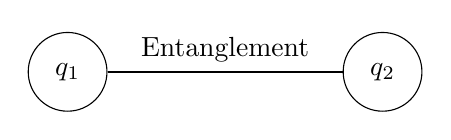
\begin{tikzpicture}
        % Nodes
        \node[circle, draw, minimum size=1cm] (q1) at (0,0) {\( q_1 \)};
        \node[circle, draw, minimum size=1cm] (q2) at (4,0) {\( q_2 \)};
        % Connection
        \draw[thick] (q1) -- (q2) node[midway, above] {Entanglement};
    \end{tikzpicture}
    \caption{Illustration of entangled qubits \( q_1 \) and \( q_2 \).}
\end{figure}

\subsection{Quantum Interference} 
Quantum interference arises from the wave-like nature of quantum particles. When quantum states overlap, their probability amplitudes can interfere constructively or destructively. Constructive interference amplifies the probability of correct solutions, while destructive interference cancels out incorrect ones. For example, in a quantum algorithm, the interference can be represented as:
\[
|\psi\rangle = \frac{1}{\sqrt{2}} \left( |0\rangle + |1\rangle \right) + \frac{1}{\sqrt{2}} \left( |0\rangle - |1\rangle \right) = |0\rangle.
\]

\begin{figure}[H]
    \centering
    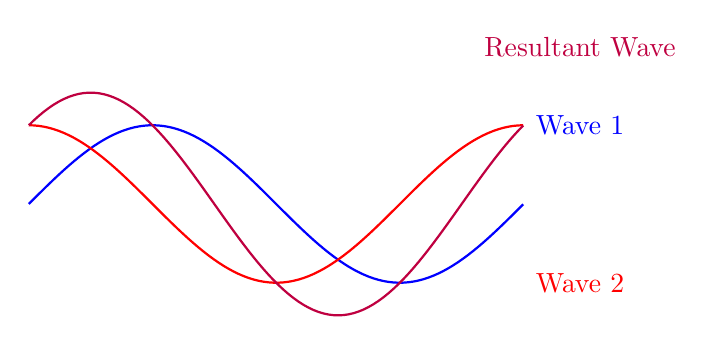
\begin{tikzpicture}
        % Waves
        \draw[thick, blue, domain=0:6.28, samples=100] plot (\x, {sin(\x r)});
        \draw[thick, red, domain=0:6.28, samples=100] plot (\x, {cos(\x r)});
        \draw[thick, purple, domain=0:6.28, samples=100] plot (\x, {sin(\x r) + cos(\x r)});
        % Labels
        \node[blue] at (7, 1) {Wave 1};
        \node[red] at (7, -1) {Wave 2};
        \node[purple] at (7, 2) {Resultant Wave};
    \end{tikzpicture}
    \caption{Constructive interference of quantum states.}
\end{figure}

\subsection{Measurement and Wavefunction Collapse}
Measurement in quantum mechanics is the process of observing a quantum system, which causes the system to collapse into a definite state. Before measurement, a quantum system exists in a superposition of all possible states, each with a certain probability amplitude. Upon measurement, the system randomly collapses into one of these states. For example, measuring the state:
\[
|\psi\rangle = \frac{1}{\sqrt{2}} |0\rangle + \frac{1}{\sqrt{2}} |1\rangle,
\]
will yield \( |0\rangle \) or \( |1\rangle \) with equal probability \( \frac{1}{2} \).

\begin{figure}[H]
    \centering
    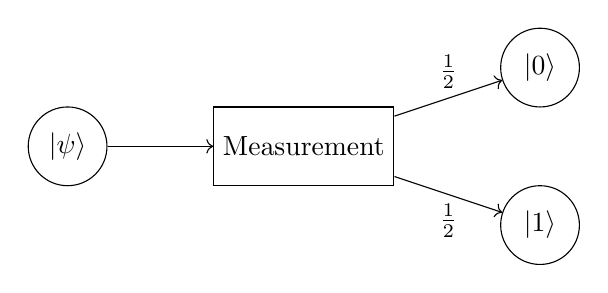
\begin{tikzpicture}
        % Qubit
        \node[circle, draw, minimum size=1cm] (qubit) at (0,0) {\( |\psi\rangle \)};
        % Measurement
        \node[rectangle, draw, minimum width=2cm, minimum height=1cm] (measure) at (3,0) {Measurement};
        % Outcomes
        \node[circle, draw, minimum size=1cm] (out1) at (6,1) {\( |0\rangle \)};
        \node[circle, draw, minimum size=1cm] (out2) at (6,-1) {\( |1\rangle \)};
        % Arrows
        \draw[->] (qubit) -- (measure);
        \draw[->] (measure) -- (out1) node[midway, above] {\( \frac{1}{2} \)};
        \draw[->] (measure) -- (out2) node[midway, below] {\( \frac{1}{2} \)};
    \end{tikzpicture}
    \caption{Measurement collapsing a qubit into a definite state.}
\end{figure}

\subsection{Quantum Tunneling} 
Quantum tunneling is a phenomenon where a quantum particle can pass through a potential energy barrier, even if it does not have enough energy to overcome it classically. This is due to the wave-like nature of quantum particles, which allows their wave functions to extend into regions that are classically forbidden. For example, the probability of tunneling through a barrier can be represented as:
\[
T \approx e^{-2\kappa L},
\]
where \( T \) is the transmission probability, \( \kappa \) is a constant related to the barrier height, and \( L \) is the barrier width.

\begin{figure}[H]
    \centering
    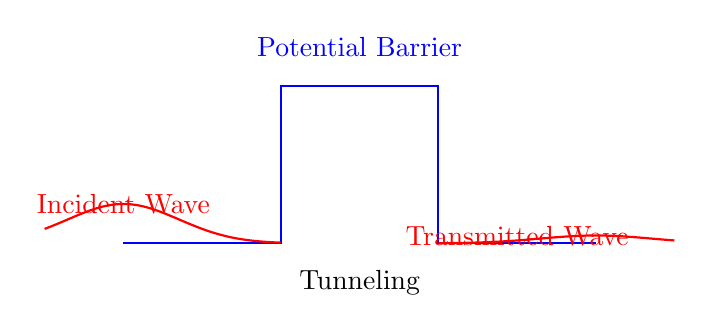
\begin{tikzpicture}
        % Potential barrier
        \draw[thick, blue] (0,0) -- (2,0) -- (2,2) -- (4,2) -- (4,0) -- (6,0);
        % Particle wave function
        \draw[thick, red, domain=-1:2, samples=100] plot (\x, {0.5*exp(-(\x-0)^2)});
        \draw[thick, red, domain=4:7, samples=100] plot (\x, {0.1*exp(-(\x-6)^2)});
        % Labels
        \node[blue] at (3, 2.5) {Potential Barrier};
        \node[red] at (0, 0.5) {Incident Wave};
        \node[red] at (5, 0.1) {Transmitted Wave};
        \node at (3, -0.5) {Tunneling};
    \end{tikzpicture}
    \caption{Quantum tunneling through a potential barrier.}
\end{figure}


\section{Mathematical Framework of Quantum Mechanics}
The mathematical framework of quantum mechanics is based on linear algebra and complex vector spaces. The key notations and concepts include:
\begin{itemize}

    \item \textbf{Schrödinger Equation:} The time evolution of a quantum system is governed by the Schrödinger equation:
    \[
    i\hbar \frac{\partial}{\partial t} |\psi(t)\rangle = \hat{H} |\psi(t)\rangle,
    \]
    where \( \hat{H} \) is the Hamiltonian operator representing the total energy of the system.

    \item \textbf{Probability Amplitudes:} The probability of measuring a particular outcome is given by the square of the amplitude of the corresponding state vector component. For example, the probability of measuring \( |0\rangle \) in the state \( |\psi\rangle = \alpha |0\rangle + \beta |1\rangle \) is \( |\alpha|^2 \).
    
    \item \textbf{State Vectors:} The state of a quantum system is represented by a vector in a complex Hilbert space, denoted as \( |\psi\rangle \). For example, a single qubit state can be written as:
    \[
    |\psi\rangle = \alpha |0\rangle + \beta |1\rangle,
    \]
    where \( \alpha, \beta \in \mathbb{C} \) and \( |\alpha|^2 + |\beta|^2 = 1 \).

    \item \textbf{Bra-Ket Notation:} Quantum states are expressed using Dirac's bra-ket notation:
    \begin{itemize}
        \item \( |\psi\rangle \): A column vector (ket) representing the state.
        \item \( \langle\psi| \): A row vector (bra), the Hermitian conjugate of \( |\psi\rangle \).
    \end{itemize}
    The inner product of two states \( |\psi\rangle \) and \( |\phi\rangle \) is written as \( \langle\psi|\phi\rangle \), and the outer product is \( |\psi\rangle\langle\phi| \).

    \item \textbf{Operators:} Physical observables, such as position and momentum, are represented by Hermitian operators acting on state vectors. For example, the Pauli-X operator is:
    \[
    X = \begin{bmatrix}
    0 & 1 \\
    1 & 0
    \end{bmatrix}.
    \]

    \item \textbf{Tensor Products:} Multi-qubit systems are represented using tensor products. For example, the state of two qubits \( |\psi_1\rangle \) and \( |\psi_2\rangle \) is:
    \[
    |\psi\rangle = |\psi_1\rangle \otimes |\psi_2\rangle.
    \]

    \item \textbf{Unitary Operators:} Quantum gates are represented by unitary matrices \( U \), satisfying \( U^\dagger U = I \), where \( U^\dagger \) is the conjugate transpose of \( U \) and \( I \) is the identity matrix.
\end{itemize}

\section{Quantum Gates and Circuits}
Quantum gates are the building blocks of quantum circuits, analogous to classical logic gates. They manipulate qubits and perform operations based on the principles of quantum mechanics:

\subsection{Single-Qubit Gates}
Single-qubit gates operate on a single qubit and are represented by \( 2 \times 2 \) unitary matrices. Examples include:
\begin{itemize}
    \item \textbf{Pauli-X Gate:} Acts as a quantum NOT gate, flipping the state of a qubit. Its matrix representation is:
    \[
    X = \begin{bmatrix}
    0 & 1 \\
    1 & 0
    \end{bmatrix}.
    \]
    \item \textbf{Hadamard Gate:} Creates a superposition of states. Its matrix representation is:
    \[
    H = \frac{1}{\sqrt{2}} \begin{bmatrix}
    1 & 1 \\
    1 & -1
    \end{bmatrix}.
    \]
    \item \textbf{Phase Gate:} Introduces a phase shift. For example, the \( S \)-gate is:
    \[
    S = \begin{bmatrix}
    1 & 0 \\
    0 & i
    \end{bmatrix}.
    \]
\end{itemize}

\subsection{Multi-Qubit Gates}
Multi-qubit gates operate on multiple qubits and are essential for creating entanglement and performing complex quantum operations:
\begin{itemize}
    \item \textbf{CNOT Gate:} A controlled-NOT gate flips the target qubit if the control qubit is \( |1\rangle \). Its matrix representation is:
    \[
    \text{CNOT} = \begin{bmatrix}
    1 & 0 & 0 & 0 \\
    0 & 1 & 0 & 0 \\
    0 & 0 & 0 & 1 \\
    0 & 0 & 1 & 0
    \end{bmatrix}.
    \]
    \item \textbf{Toffoli Gate:} A controlled-controlled-NOT gate, which flips the target qubit if both control qubits are \( |1\rangle \).
\end{itemize}

\subsection{Quantum Circuits}
A quantum circuit is a sequence of quantum gates applied to qubits to perform a computation. Mathematically, the overall operation of a quantum circuit is represented by the product of the unitary matrices of its gates. The output is obtained by measuring the qubits, collapsing their states into classical bits.

\section{Relevance to Quantum Computing}
Quantum mechanics provides the theoretical underpinnings for quantum computing, enabling the development of powerful algorithms. For example:
\begin{itemize}
    \item \textbf{Shor's Algorithm:} Efficiently factors integers by leveraging quantum Fourier transforms.
    \item \textbf{Grover's Algorithm:} Provides a quadratic speedup for unstructured search problems.
\end{itemize}
By leveraging principles such as superposition, entanglement, and interference, quantum computers can solve problems that are intractable for classical computers.

\section{Challenges in Quantum Mechanics for Computing}
Despite its potential, quantum mechanics introduces challenges for quantum computing:
\begin{itemize}
    \item \textbf{Decoherence:} Quantum states are fragile and can lose coherence due to interactions with the environment, leading to errors in computation.
    \item \textbf{Error Correction:} Quantum error correction codes, such as the surface code, are required to mitigate the effects of noise and decoherence. These codes rely on encoding logical qubits into multiple physical qubits.
    \item \textbf{Scalability:} Building large-scale quantum computers with many qubits while maintaining coherence and low error rates is a complex engineering problem.
\end{itemize}

This chapter establishes the connection between quantum mechanics and quantum computing, highlighting the transformative potential of this interdisciplinary field and the challenges that must be overcome to realize its full potential.

\chapter{Existing Methods for Breaking RSA Before Quantum Computing}
\label{chap:existing_methods}
Before the advent of quantum computing, several classical methods were explored to break RSA encryption. These methods, while not as efficient as quantum algorithms, posed potential threats under certain conditions. This chapter discusses the existing systems and techniques used to attack RSA encryption prior to the emergence of quantum computing.

\section{Brute Force Attacks}
Brute force attacks involve systematically trying all possible private keys to decrypt a message. However, due to the large key sizes used in RSA (typically 2048 bits or more), brute force attacks are computationally infeasible with classical computers.

\section{Mathematical Factorization Algorithms}
The security of RSA relies on the difficulty of factoring large integers. Several classical algorithms have been developed to factorize numbers, including:
\begin{itemize}
    \item \textbf{Trial Division:} A basic method that tests divisibility by smaller numbers, but it is highly inefficient for large integers.
    \item \textbf{Pollard's Rho Algorithm:} A probabilistic algorithm that works well for smaller numbers but struggles with large RSA keys.
    \item \textbf{Quadratic Sieve:} One of the fastest classical algorithms for factoring integers up to 100 digits.
    \item \textbf{General Number Field Sieve (GNFS):} The most efficient classical algorithm for factoring large integers, used in practical attacks on RSA with smaller key sizes.
\end{itemize}

\section{Side-Channel Attacks}
Side-channel attacks exploit physical implementations of RSA rather than its mathematical foundation. Examples include:
\begin{itemize}
    \item \textbf{Timing Attacks:} Measuring the time taken for cryptographic operations to infer private keys.
    \item \textbf{Power Analysis:} Observing power consumption patterns during encryption or decryption.
    \item \textbf{Electromagnetic Analysis:} Capturing electromagnetic emissions to extract sensitive information.
\end{itemize}

\section{Distributed Computing Efforts}
Projects like the RSA Factoring Challenge encouraged distributed computing efforts to factorize RSA keys. While these efforts demonstrated the vulnerability of smaller key sizes, they were not practical for breaking modern RSA implementations with sufficiently large keys.

\section{Limitations of Classical Methods}
Despite these methods, breaking RSA encryption with classical computers remains infeasible for adequately large key sizes. The computational resources and time required grow exponentially with key size, ensuring the security of RSA against classical attacks.

While RSA encryption has been a reliable cryptographic standard, it is not without limitations. The primary challenge lies in its reliance on the difficulty of integer factorization. With the advent of quantum computing, this foundational assumption is under threat, as quantum algorithms like Shor's algorithm can efficiently solve the integer factorization problem.

\chapter{Drawbacks of Existing Methods}
While existing methods for breaking RSA encryption have been extensively studied, they come with significant drawbacks that limit their practicality and effectiveness. This chapter discusses the key limitations of these methods:

\section{Brute Force Attacks}
\begin{itemize}
    \item \textbf{Exponential Time Complexity:} The time required to test all possible keys grows exponentially with key size, making brute force attacks infeasible for modern RSA implementations.
    \item \textbf{Resource Intensive:} Brute force attacks require substantial computational resources, which are often unavailable or impractical to deploy.
\end{itemize}

\section{Mathematical Factorization Algorithms}
\begin{itemize}
    \item \textbf{Inefficiency for Large Keys:} Classical factorization algorithms, such as the General Number Field Sieve (GNFS), become increasingly inefficient as the size of the RSA key increases.
    \item \textbf{High Computational Cost:} These algorithms demand significant computational power and time, limiting their applicability to smaller key sizes.
\end{itemize}

\section{Side-Channel Attacks}
\begin{itemize}
    \item \textbf{Dependency on Physical Access:} Side-channel attacks often require physical access to the cryptographic device, which is not always feasible.
    \item \textbf{Mitigation Techniques:} Modern cryptographic implementations include countermeasures to reduce the effectiveness of side-channel attacks, such as constant-time algorithms and noise injection.
\end{itemize}

\section{Distributed Computing Efforts}
\begin{itemize}
    \item \textbf{Scalability Issues:} Distributed computing efforts face challenges in scaling to factorize larger RSA keys due to the exponential growth in computational requirements.
    \item \textbf{Coordination Overhead:} Managing and coordinating large-scale distributed systems introduces additional complexity and overhead.
\end{itemize}

\section{General Limitations}
\begin{itemize}
    \item \textbf{Reliance on Classical Computing:} All existing methods are constrained by the limitations of classical computing, which cannot efficiently solve the integer factorization problem for large key sizes.
    \item \textbf{Inability to Address Quantum Threats:} These methods do not account for the advancements in quantum computing, which pose a more significant threat to RSA encryption.
\end{itemize}

These drawbacks highlight the need for more advanced approaches, such as quantum-resistant cryptographic systems, to address the vulnerabilities of RSA encryption in the face of evolving computational capabilities.

\chapter{Shor's Algorithm and Its Impact on RSA}
\label{chap:shors_algorithm}
Shor's algorithm is a quantum algorithm that can factorize large integers exponentially faster than classical algorithms. This chapter delves into the workings of Shor's algorithm and explains how it directly undermines the security of RSA encryption, making it vulnerable to quantum attacks.

\chapter{Implications of Quantum Computing on Cryptography}
The ability of quantum computers to break RSA encryption has far-reaching implications for cryptography. This chapter discusses the potential risks to digital security, including compromised financial transactions, data breaches, and threats to national security, emphasizing the urgency of addressing these challenges.

\chapter{Advantages of Proposed System}
The proposed quantum-resistant cryptographic systems offer several advantages:
\begin{itemize}
    \item Enhanced security against quantum attacks, ensuring the confidentiality of sensitive information.
    \item Compatibility with existing communication protocols, allowing for a smoother transition to quantum-resistant systems.
    \item Scalability for future cryptographic needs, addressing the growing demand for secure communication in the quantum era.
    \item Reduced risk of data breaches and financial fraud caused by quantum-enabled attacks.
\end{itemize}

\chapter{Application}
Quantum-resistant cryptographic systems have a wide range of applications, including:
\begin{itemize}
    \item Securing financial transactions and online banking systems.
    \item Protecting sensitive government and military communications.
    \item Ensuring the privacy of personal data in healthcare and other industries.
    \item Safeguarding intellectual property and trade secrets in the corporate sector.
    \item Enabling secure communication in emerging technologies such as the Internet of Things (IoT) and autonomous vehicles.
\end{itemize}

\chapter{Future Enhancement and Research Directions in Quantum Computing}
The field of quantum computing is rapidly evolving, with ongoing research and development efforts to overcome existing challenges and enhance the capabilities of quantum systems. 

\section{Current State of Quantum Computing Technology}
\label{sec:challenge_quantum_computing}
The threat posed by quantum computing to RSA encryption is based on Shor's algorithm, which can efficiently factorize large integers. However, the practical realization of this threat depends on the current state of quantum computing technology. Several challenges limit the immediate impact of quantum computing on RSA encryption:

\begin{itemize}
    \item \textbf{Qubit Stability:} Quantum computers require stable qubits to perform reliable computations. Current quantum systems face challenges in maintaining qubit coherence and stability over extended periods.
    \item \textbf{Error Rates:} Quantum operations are susceptible to errors due to noise and environmental factors. Error correction techniques are essential to mitigate these errors and ensure the accuracy of quantum computations.
    \item \textbf{Scalability:} Building large-scale quantum computers with thousands of qubits is a complex engineering feat. Scaling quantum systems while maintaining coherence and low error rates remains a significant challenge.
    \item \textbf{Error Correction:} Quantum error correction codes are essential to protect quantum information from errors. Implementing error correction at scale is a non-trivial task that requires significant computational resources.
    \item \textbf{Algorithmic Improvements:} While Shor's algorithm demonstrates the theoretical threat to RSA encryption, practical implementations require further algorithmic improvements and optimizations to factorize large integers efficiently.
\end{itemize}

While the theoretical threat posed by Shor's algorithm is significant, the current state of quantum computing technology is not yet advanced enough to break RSA encryption with commonly used key lengths like 2048 bits~\cite{SpinQShor}. Current quantum computers are still in the early stages of development and face limitations in the number of stable and error-corrected qubits (quantum bits) they possess~\cite{CatoNetworks}.

Estimates for the number of logical qubits required to break RSA-2048 vary, ranging from around 4,000 to 20 million, depending on the specific algorithm implementation and assumptions about error correction~\cite{BTQHowFar}. The largest number factored using Shor's algorithm on a quantum computer to date is 21~\cite{SpinQShor}. While there have been claims of breaking larger RSA keys using hybrid quantum-classical approaches with fewer qubits, these have generally involved significantly smaller key sizes (e.g., 22 bits) and do not yet pose a threat to standard RSA implementations~\cite{FreemindtronicRSA}.

\section{Quantum-Resistant Cryptography}
Quantum-resistant cryptography, also known as post-quantum cryptography, aims to develop cryptographic algorithms that are secure against both classical and quantum computers. These algorithms are based on mathematical problems that are believed to be resistant to quantum attacks, such as lattice-based cryptography, hash-based cryptography, code-based cryptography, and multivariate polynomial cryptography.

\subsection{Standardization Efforts}
Organizations like NIST (National Institute of Standards and Technology) are actively working on standardizing quantum-resistant algorithms. The NIST Post-Quantum Cryptography Standardization project has identified several candidate algorithms for public-key encryption, digital signatures, and key exchange protocols. These efforts aim to ensure global adoption and interoperability of quantum-resistant cryptographic systems.

\subsection{Challenges and Research Directions}
While quantum-resistant cryptography holds promise, several challenges remain:
\begin{itemize}
    \item \textbf{Performance Overhead:} Quantum-resistant algorithms often require larger key sizes and computational resources compared to traditional cryptographic systems.
    \item \textbf{Security Analysis:} Extensive research is needed to analyze the security of proposed algorithms against both classical and quantum attacks.
    \item \textbf{Integration with Existing Systems:} Transitioning to quantum-resistant cryptography requires compatibility with existing communication protocols and infrastructure.
\end{itemize}

\subsection{Future Enhancements}
The advent of quantum computing poses a significant challenge to traditional cryptographic systems like RSA encryption. However, it also drives innovation in the field of cryptography, leading to the development of quantum-resistant algorithms. Future enhancements in this area include:
\begin{itemize}
    \item Standardizing quantum-resistant algorithms to ensure global adoption and interoperability.
    \item Improving the efficiency and performance of quantum-resistant cryptographic systems to meet real-world demands.
    \item Conducting extensive research to identify and mitigate potential vulnerabilities in proposed systems.
\end{itemize}


\chapter{Conclusion}
In conclusion, the transition to quantum-resistant cryptography is essential to mitigate the risks posed by quantum computing. By adopting these advanced systems, we can ensure the continued security of sensitive information and maintain trust in digital communication in the quantum era.

\begin{thebibliography}{50}
    \bibitem{Rivest1978}
    Rivest, R., Shamir, A., \& Adleman, L. (1978). 
    \textit{A Method for Obtaining Digital Signatures and Public-Key Cryptosystems}. 
    Communications of the ACM, 21(2), 120--126. 
    doi:\href{https://doi.org/10.1145/359340.359342}{10.1145/359340.359342}.
    CiteSeerX: \href{https://citeseerx.ist.psu.edu/viewdoc/summary?doi=10.1.1.607.2677}{10.1.1.607.2677}.
    S2CID: \href{https://scite.ai/reports/2873616}{2873616}.
    Archived from the original (PDF) on 2023--01--27.\@ 
    Available at: \url{http://people.csail.mit.edu/rivest/Rsapaper.pdf}.
    
    \bibitem{Okta}
    Okta. (2025). 
    \textit{RSA Encryption: Definition, Architecture, Benefits \& Use}. 
    Retrieved March 23, 2025, from \url{https://www.okta.com/identity-101/rsa-encryption/}.
    
    \bibitem{SecureW2}
    SecureW2. (2025). 
    \textit{Understanding RSA Asymmetric Encryption: How It Works}. 
    Retrieved March 23, 2025, from \url{https://www.securew2.com/blog/what-is-rsa-asymmetric-encryption}.
    
    \bibitem{SoftwareDominos}
    SoftwareDominos. (2025). 
    \textit{Understanding RSA: The Mathematics Behind Secure Encryption}. 
    Retrieved March 23, 2025, from \url{https://softwaredominos.com/home/software-engineering-and-computer-science/understanding-rsa-the-mathematics-behind-secure-encryption/}.
    
    \bibitem{RSAWiki}
    Wikipedia. (2025). 
    \textit{RSA problem}. 
    Retrieved March 23, 2025, from \url{https://en.wikipedia.org/wiki/RSA_problem}.
    
    \bibitem{ODUCommons}
    ODU Digital Commons. (2025). 
    \textit{The Vulnerabilities to the RSA Algorithm and Future Alternative Algorithms to Improve Security}. 
    Retrieved March 23, 2025, from \url{https://digitalcommons.odu.edu/cgi/viewcontent.cgi?article=1081&context=covacci-undergraduateresearch}.
    
    \bibitem{AuthoreaImplementation}
    Authorea. (2025).
    \textit{Implementation and Analysis of Shor's Algorithm to Break RSA Cryptosystem Security}.
    Retrieved March 23, 2025, from \url{https://www.authorea.com/users/708580/articles/693052-implementation-and-analysis-of-shor-s-algorithm-to-break-rsa-cryptosystem-security}.
    
    \bibitem{SpinQShor}
    SpinQ. (2025).
    \textit{How Shor's Algorithm Breaks RSA: A Quantum Computing Guide}.
    Retrieved March 23, 2025, from \url{https://www.spinquanta.com/news-detail/shors-algorithm}.
    
    \bibitem{GeeksForGeeks}
    GeeksforGeeks. (2025).
    \textit{RSA Algorithm in Cryptography}.
    Retrieved March 23, 2025, from \url{https://www.geeksforgeeks.org/rsa-algorithm-cryptography/}.
    
    \bibitem{SplunkRSA}
    Splunk. (2025).
    \textit{RSA Algorithm in Cryptography: Rivest Shamir Adleman Explained}.
    Retrieved March 23, 2025, from \url{https://www.splunk.com/en_us/blog/learn/rsa-algorithm-cryptography.html}.
    
    \bibitem{TechRxivImplementation}
    TechRxiv. (2025).
    \textit{Implementation and Analysis of Shor's Algorithm to Break RSA Cryptosystem Security}.
    Retrieved March 23, 2025, from \url{https://www.techrxiv.org/users/708580/articles/693052/master/file/data/RESERCH%20FINAL/RESERCH%20FINAL.pdf}.
    
    \bibitem{ResearchGateImplementation}
    ResearchGate. (2025).
    \textit{Implementation and Analysis of Shor's Algorithm to Break RSA Cryptosystem Security}.
    Retrieved March 23, 2025, from \url{https://www.researchgate.net/publication/377245624_Implementation_and_Analysis_of_Shor's_Algorithm_to_Break_RSA_Cryptosystem_Security}.
    
    \bibitem{CatoNetworks}
    Cato Networks. (2025).
    \textit{Is the Recent Quantum Hype by Google Willow's Chip a Threat to RSA Algorithm?}
    Retrieved March 23, 2025, from \url{https://www.catonetworks.com/blog/is-recent-quantum-hype-by-google-willows-chip-a-threat-to-rsa-algorithm/}.
    
    \bibitem{BTQHowFar}
    BTQ. (2025).
    \textit{How Far Away Is The Quantum Threat?}
    Retrieved March 23, 2025, from \url{https://www.btq.com/blog/how-far-away-is-the-quantum-threat}.
    
    \bibitem{FreemindtronicRSA}
    Freemindtronic. (2025).
    \textit{Quantum computing RSA encryption: a threat and a solution}.
    Retrieved March 23, 2025, from \url{https://freemindtronic.com/quantum-computing-rsa-encryption-freemindtronic-nfc-technology/}.
    
    \bibitem{PaloAltoNetworks}
    Palo Alto Networks. (2025).
    \textit{What Is Quantum Computing's Threat to Cybersecurity?}
    Retrieved March 23, 2025, from \url{https://www.paloaltonetworks.com/cyberpedia/what-is-quantum-computings-threat-to-cybersecurity}.
    
    \bibitem{IBMCommunity}
    IBM Community. (2025).
    \textit{How many Number of qubits required for decryption}.
    Retrieved March 23, 2025, from \url{https://community.ibm.com/community/user/ai-datascience/discussion/how-many-number-of-qubits-required-for-decryption}.
    
    \bibitem{SectigoConcerns}
    Sectigo. (2025).
    \textit{Quantum computing concerns \& positive impacts}.
    Retrieved March 23, 2025, from \url{https://www.sectigo.com/resource-library/quantum-computing-concerns-positive-impacts}.
    
    \bibitem{NISTPQC}
    NIST Computer Security Resource Center. (2025).
    \textit{Post-Quantum Cryptography}.
    Retrieved March 23, 2025, from \url{https://csrc.nist.gov/projects/post-quantum-cryptography}.
    
    \bibitem{NISTStandardization}
    Wikipedia. (2025).
    \textit{NIST Post-Quantum Cryptography Standardization}.
    Retrieved March 23, 2025, from \url{https://en.wikipedia.org/wiki/NIST_Post-Quantum_Cryptography_Standardization}.
    
    \bibitem{GooglePQC}
    Google Online Security Blog. (2024).
    \textit{Post-Quantum Cryptography: Standards and Progress}.
    Retrieved March 23, 2025, from \url{https://security.googleblog.com/2024/08/post-quantum-cryptography-standards.html}.
\end{thebibliography}

\end{document}